\documentclass[]{article}
\usepackage{lmodern}
\usepackage{amssymb,amsmath}
\usepackage{ifxetex,ifluatex}
\usepackage{fixltx2e} % provides \textsubscript
\ifnum 0\ifxetex 1\fi\ifluatex 1\fi=0 % if pdftex
  \usepackage[T1]{fontenc}
  \usepackage[utf8]{inputenc}
\else % if luatex or xelatex
  \ifxetex
    \usepackage{mathspec}
  \else
    \usepackage{fontspec}
  \fi
  \defaultfontfeatures{Ligatures=TeX,Scale=MatchLowercase}
\fi
% use upquote if available, for straight quotes in verbatim environments
\IfFileExists{upquote.sty}{\usepackage{upquote}}{}
% use microtype if available
\IfFileExists{microtype.sty}{%
\usepackage{microtype}
\UseMicrotypeSet[protrusion]{basicmath} % disable protrusion for tt fonts
}{}
\usepackage[margin=1in]{geometry}
\usepackage{hyperref}
\hypersetup{unicode=true,
            pdftitle={Robustness checks},
            pdfauthor={Falco J. Bargagli-Stoffi, Massimo Riccaboni, Armando Rungi},
            pdfborder={0 0 0},
            breaklinks=true}
\urlstyle{same}  % don't use monospace font for urls
\usepackage{color}
\usepackage{fancyvrb}
\newcommand{\VerbBar}{|}
\newcommand{\VERB}{\Verb[commandchars=\\\{\}]}
\DefineVerbatimEnvironment{Highlighting}{Verbatim}{commandchars=\\\{\}}
% Add ',fontsize=\small' for more characters per line
\usepackage{framed}
\definecolor{shadecolor}{RGB}{248,248,248}
\newenvironment{Shaded}{\begin{snugshade}}{\end{snugshade}}
\newcommand{\AlertTok}[1]{\textcolor[rgb]{0.94,0.16,0.16}{#1}}
\newcommand{\AnnotationTok}[1]{\textcolor[rgb]{0.56,0.35,0.01}{\textbf{\textit{#1}}}}
\newcommand{\AttributeTok}[1]{\textcolor[rgb]{0.77,0.63,0.00}{#1}}
\newcommand{\BaseNTok}[1]{\textcolor[rgb]{0.00,0.00,0.81}{#1}}
\newcommand{\BuiltInTok}[1]{#1}
\newcommand{\CharTok}[1]{\textcolor[rgb]{0.31,0.60,0.02}{#1}}
\newcommand{\CommentTok}[1]{\textcolor[rgb]{0.56,0.35,0.01}{\textit{#1}}}
\newcommand{\CommentVarTok}[1]{\textcolor[rgb]{0.56,0.35,0.01}{\textbf{\textit{#1}}}}
\newcommand{\ConstantTok}[1]{\textcolor[rgb]{0.00,0.00,0.00}{#1}}
\newcommand{\ControlFlowTok}[1]{\textcolor[rgb]{0.13,0.29,0.53}{\textbf{#1}}}
\newcommand{\DataTypeTok}[1]{\textcolor[rgb]{0.13,0.29,0.53}{#1}}
\newcommand{\DecValTok}[1]{\textcolor[rgb]{0.00,0.00,0.81}{#1}}
\newcommand{\DocumentationTok}[1]{\textcolor[rgb]{0.56,0.35,0.01}{\textbf{\textit{#1}}}}
\newcommand{\ErrorTok}[1]{\textcolor[rgb]{0.64,0.00,0.00}{\textbf{#1}}}
\newcommand{\ExtensionTok}[1]{#1}
\newcommand{\FloatTok}[1]{\textcolor[rgb]{0.00,0.00,0.81}{#1}}
\newcommand{\FunctionTok}[1]{\textcolor[rgb]{0.00,0.00,0.00}{#1}}
\newcommand{\ImportTok}[1]{#1}
\newcommand{\InformationTok}[1]{\textcolor[rgb]{0.56,0.35,0.01}{\textbf{\textit{#1}}}}
\newcommand{\KeywordTok}[1]{\textcolor[rgb]{0.13,0.29,0.53}{\textbf{#1}}}
\newcommand{\NormalTok}[1]{#1}
\newcommand{\OperatorTok}[1]{\textcolor[rgb]{0.81,0.36,0.00}{\textbf{#1}}}
\newcommand{\OtherTok}[1]{\textcolor[rgb]{0.56,0.35,0.01}{#1}}
\newcommand{\PreprocessorTok}[1]{\textcolor[rgb]{0.56,0.35,0.01}{\textit{#1}}}
\newcommand{\RegionMarkerTok}[1]{#1}
\newcommand{\SpecialCharTok}[1]{\textcolor[rgb]{0.00,0.00,0.00}{#1}}
\newcommand{\SpecialStringTok}[1]{\textcolor[rgb]{0.31,0.60,0.02}{#1}}
\newcommand{\StringTok}[1]{\textcolor[rgb]{0.31,0.60,0.02}{#1}}
\newcommand{\VariableTok}[1]{\textcolor[rgb]{0.00,0.00,0.00}{#1}}
\newcommand{\VerbatimStringTok}[1]{\textcolor[rgb]{0.31,0.60,0.02}{#1}}
\newcommand{\WarningTok}[1]{\textcolor[rgb]{0.56,0.35,0.01}{\textbf{\textit{#1}}}}
\usepackage{graphicx,grffile}
\makeatletter
\def\maxwidth{\ifdim\Gin@nat@width>\linewidth\linewidth\else\Gin@nat@width\fi}
\def\maxheight{\ifdim\Gin@nat@height>\textheight\textheight\else\Gin@nat@height\fi}
\makeatother
% Scale images if necessary, so that they will not overflow the page
% margins by default, and it is still possible to overwrite the defaults
% using explicit options in \includegraphics[width, height, ...]{}
\setkeys{Gin}{width=\maxwidth,height=\maxheight,keepaspectratio}
\IfFileExists{parskip.sty}{%
\usepackage{parskip}
}{% else
\setlength{\parindent}{0pt}
\setlength{\parskip}{6pt plus 2pt minus 1pt}
}
\setlength{\emergencystretch}{3em}  % prevent overfull lines
\providecommand{\tightlist}{%
  \setlength{\itemsep}{0pt}\setlength{\parskip}{0pt}}
\setcounter{secnumdepth}{0}
% Redefines (sub)paragraphs to behave more like sections
\ifx\paragraph\undefined\else
\let\oldparagraph\paragraph
\renewcommand{\paragraph}[1]{\oldparagraph{#1}\mbox{}}
\fi
\ifx\subparagraph\undefined\else
\let\oldsubparagraph\subparagraph
\renewcommand{\subparagraph}[1]{\oldsubparagraph{#1}\mbox{}}
\fi

%%% Use protect on footnotes to avoid problems with footnotes in titles
\let\rmarkdownfootnote\footnote%
\def\footnote{\protect\rmarkdownfootnote}

%%% Change title format to be more compact
\usepackage{titling}

% Create subtitle command for use in maketitle
\providecommand{\subtitle}[1]{
  \posttitle{
    \begin{center}\large#1\end{center}
    }
}

\setlength{\droptitle}{-2em}

  \title{Robustness checks}
    \pretitle{\vspace{\droptitle}\centering\huge}
  \posttitle{\par}
    \author{Falco J. Bargagli-Stoffi, Massimo Riccaboni, Armando Rungi}
    \preauthor{\centering\large\emph}
  \postauthor{\par}
      \predate{\centering\large\emph}
  \postdate{\par}
    \date{25/2/2020}


\begin{document}
\maketitle

\hypertarget{introduction}{%
\section{Introduction}\label{introduction}}

This \texttt{R Markdown} file reproduces the robustness check analyses
for the paper
\textit{"Machine learning for zombie hunting. Firms' failures, financial constraints, and misallocation"}
by Falco J. Bargagli-Stoffi (IMT School for Advanced Studies/KU Leuven),
Massimo Riccaboni (IMT School for Advanced Studies) and Armando Rungi
(IMT School for Advanced Studies).

\hypertarget{r-markdown}{%
\subsection{R Markdown}\label{r-markdown}}

This is an \texttt{R Markdown} document. Markdown is a simple formatting
syntax for authoring HTML, PDF, and MS Word documents. For more details
on using \texttt{R Markdown} see \url{http://rmarkdown.rstudio.com}.

When you click the \textbf{Knit} button a document will be generated
that includes both content as well as the output of any embedded
\texttt{R} code chunks within the document. You can embed an R code
chunks like the following.

\hypertarget{packages-upload}{%
\subsection{Packages Upload}\label{packages-upload}}

The following packages and functions are the ones used for the analyses
performed in the \texttt{R} code. The \texttt{functions.R} file contains
the functions \texttt{F1\_score}, \texttt{balanced\_accuracy},
\texttt{model\_compare} and \texttt{DtD} that were developed to
reproduce the following analyses.

\begin{Shaded}
\begin{Highlighting}[]
\KeywordTok{rm}\NormalTok{(}\DataTypeTok{list=}\KeywordTok{ls}\NormalTok{()) }\CommentTok{# to clean the memeory}
\KeywordTok{memory.limit}\NormalTok{(}\DataTypeTok{size=}\DecValTok{1000000}\NormalTok{)}
\end{Highlighting}
\end{Shaded}

\begin{verbatim}
## [1] 1e+06
\end{verbatim}

\begin{Shaded}
\begin{Highlighting}[]
\KeywordTok{options}\NormalTok{(}\DataTypeTok{java.parameters =} \StringTok{"-Xmx15000m"}\NormalTok{)}
\KeywordTok{library}\NormalTok{(haven)}
\KeywordTok{library}\NormalTok{(BART)}
\KeywordTok{library}\NormalTok{(ggplot2)}
\KeywordTok{source}\NormalTok{(}\StringTok{'sensitivity.R'}\NormalTok{)}
\end{Highlighting}
\end{Shaded}

\hypertarget{data-upload}{%
\subsection{Data Upload}\label{data-upload}}

In the following chunks of code we upload the data, we initialize the
main variables used in the analysis and we restrict the sample to the
Italian firms.

\begin{Shaded}
\begin{Highlighting}[]
\NormalTok{data <-}\StringTok{ }\KeywordTok{read_dta}\NormalTok{(}\StringTok{"analysis_data_indicators.dta"}\NormalTok{)}
\end{Highlighting}
\end{Shaded}

\begin{Shaded}
\begin{Highlighting}[]
\KeywordTok{names}\NormalTok{(data)[}\KeywordTok{names}\NormalTok{(data) }\OperatorTok{==}\StringTok{ 'GUO___BvD_ID_number'}\NormalTok{] <-}\StringTok{ 'guo'}
\NormalTok{data}\OperatorTok{$}\NormalTok{control <-}\StringTok{ }\KeywordTok{ifelse}\NormalTok{(data}\OperatorTok{$}\NormalTok{guo}\OperatorTok{==}\StringTok{""}\NormalTok{, }\DecValTok{0}\NormalTok{, }\DecValTok{1}\NormalTok{)}
\NormalTok{data}\OperatorTok{$}\NormalTok{nace <-}\StringTok{ }\KeywordTok{as.factor}\NormalTok{(data}\OperatorTok{$}\NormalTok{nace)}
\NormalTok{data}\OperatorTok{$}\NormalTok{area <-}\StringTok{ }\KeywordTok{as.factor}\NormalTok{(data}\OperatorTok{$}\NormalTok{area)}
\KeywordTok{levels}\NormalTok{(data}\OperatorTok{$}\NormalTok{nace) <-}\StringTok{ }\KeywordTok{floor}\NormalTok{(}\KeywordTok{as.numeric}\NormalTok{(}\KeywordTok{levels}\NormalTok{(data}\OperatorTok{$}\NormalTok{nace))}\OperatorTok{/}\DecValTok{100}\NormalTok{) }
\NormalTok{data_italy <-}\StringTok{ }\NormalTok{data[}\KeywordTok{which}\NormalTok{(data}\OperatorTok{$}\NormalTok{iso}\OperatorTok{==}\StringTok{"IT"}\NormalTok{),] }
\end{Highlighting}
\end{Shaded}

\hypertarget{sensitivity-of-predictions-analysis}{%
\section{Sensitivity of Predictions
Analysis}\label{sensitivity-of-predictions-analysis}}

Here, we perform the ``sensitivity analysis'' for the predictions
obtained from the BART algorithm. Since these predictions are the
foundations of our paper, it is important to check whether or not they
are stable. The following sensitivity of predictions analysis comes from
a recent paper by Bargagli-Stoffi et al. (2020).

The stability of predictions is checked with respect to the unit level
predicted financial literacy scores that we get from the original model:
\begin{equation}
 f_(x) = \hat{Y}(X_i=x).
\end{equation}

\par

The ``robustness'' of the predictions is tested with respect to the
inclusion of new predictors uncorrelated with varying correlations with
the outcome.

\par

In particular, this check is performed by generating a new predictor, a
``confounder'' \(R_i\), orthogonal to the set of predictors
\(\mathbf{X}\) and with a correlation with the outcome that varies
between 0.1 and 0.4, and checking how the inclusion of this additional
predictor affects on the original model. The new model is the following:
\begin{equation}
 f_(x,r) = \hat{Y}(X_i=x, R_i=r).
\end{equation}

This check is done with respect to the following dimensions:

\begin{enumerate}
 \item percentual decrease in the bias of $f_(x,r)$ wrt $f_(x)$;
 \item percentual decrease in the RMSE of $f_(x,r)$ wrt $f_(x)$;
 \item percentual increase in the $R^2$ of $f_(x,r)$ wrt $f_(x)$;
 \item statistical difference between $\hat{Y}(x,r)$ and $\hat{Y}(x)$ at a significance level of $\alpha$.
\end{enumerate}

\par

We argue that if these differences are not wide, there is room to think
that the original model is capturing much of the signal in the data. In
this case, the original model is stable and the addition of a new
important predictor (i.e., the best predictors have roughly correlation
0.5 with the output) is not inducing substantial changes in the accuracy
measures (i.e., bias, RMSE, \(R^2\)) and, more importantly, is not
affecting in a sensible way the predicted values.

\par

Let's now see in detail how do we implement these robustness checks in
\texttt{R}.

\hypertarget{data-inizialization}{%
\subsection{Data Inizialization}\label{data-inizialization}}

Select the lagged variables and the predictors.

\begin{Shaded}
\begin{Highlighting}[]
\NormalTok{lagged_variables <-}\StringTok{ }\KeywordTok{c}\NormalTok{(}\StringTok{"failure"}\NormalTok{, }\StringTok{"iso"}\NormalTok{, }\StringTok{"control"}\NormalTok{, }\StringTok{"nace"}\NormalTok{,}
                      \StringTok{"shareholders_funds"}\NormalTok{, }\StringTok{"added_value"}\NormalTok{,}
                      \StringTok{"cash_flow"}\NormalTok{, }\StringTok{"ebitda"}\NormalTok{, }\StringTok{"fin_rev"}\NormalTok{,}
                      \StringTok{"liquidity_ratio"}\NormalTok{, }\StringTok{"total_assets"}\NormalTok{,}
                      \StringTok{"depr"}\NormalTok{, }\StringTok{"long_term_debt"}\NormalTok{, }\StringTok{"employees"}\NormalTok{,}
                      \StringTok{"materials"}\NormalTok{, }\StringTok{"loans"}\NormalTok{, }\StringTok{"wage_bill"}\NormalTok{,}
                      \StringTok{"tfp_acf"}\NormalTok{, }\StringTok{"fixed_assets"}\NormalTok{, }\StringTok{"tax"}\NormalTok{,}
                      \StringTok{"current_liabilities"}\NormalTok{, }\StringTok{"current_assets"}\NormalTok{,}
                      \StringTok{"fin_expenses"}\NormalTok{, }\StringTok{"int_paid"}\NormalTok{,}
                      \StringTok{"solvency_ratio"}\NormalTok{, }\StringTok{"net_income"}\NormalTok{,}
                      \StringTok{"revenue"}\NormalTok{, }\StringTok{"consdummy"}\NormalTok{, }\StringTok{"capital_intensity"}\NormalTok{,}
                      \StringTok{"fin_cons100"}\NormalTok{, }\StringTok{"inv"}\NormalTok{, }\StringTok{"ICR_failure"}\NormalTok{,}
                      \StringTok{"interest_diff"}\NormalTok{, }\StringTok{"NEG_VA"}\NormalTok{, }\StringTok{"real_SA"}\NormalTok{,}
                      \StringTok{"Z_score"}\NormalTok{, }\StringTok{"misallocated_fixed"}\NormalTok{,}
                      \StringTok{"profitability"}\NormalTok{, }\StringTok{"area"}\NormalTok{, }\StringTok{"dummy_patents"}\NormalTok{,}
                      \StringTok{"dummy_trademark"}\NormalTok{,}\StringTok{"financial_sustainability"}\NormalTok{,}
                      \StringTok{"liquidity_return"}\NormalTok{, }\StringTok{"int_fixed_assets"}\NormalTok{)}
\NormalTok{data_lagged <-}\StringTok{ }\NormalTok{data_italy[lagged_variables]}

\NormalTok{predictors <-}\StringTok{ }\KeywordTok{c}\NormalTok{(}\StringTok{"control"}\NormalTok{, }\StringTok{"nace"}\NormalTok{, }\StringTok{"shareholders_funds"}\NormalTok{,}
                \StringTok{"added_value"}\NormalTok{, }\StringTok{"cash_flow"}\NormalTok{, }\StringTok{"ebitda"}\NormalTok{,}
                \StringTok{"fin_rev"}\NormalTok{, }\StringTok{"liquidity_ratio"}\NormalTok{, }\StringTok{"total_assets"}\NormalTok{,}
                \StringTok{"depr"}\NormalTok{, }\StringTok{"long_term_debt"}\NormalTok{, }\StringTok{"employees"}\NormalTok{,}
                \StringTok{"materials"}\NormalTok{, }\StringTok{"loans"}\NormalTok{, }\StringTok{"wage_bill"}\NormalTok{, }\StringTok{"tfp_acf"}\NormalTok{,}
                \StringTok{"fixed_assets"}\NormalTok{, }\StringTok{"tax"}\NormalTok{, }\StringTok{"current_liabilities"}\NormalTok{,}
                \StringTok{"current_assets"}\NormalTok{, }\StringTok{"fin_expenses"}\NormalTok{, }\StringTok{"int_paid"}\NormalTok{,}
                \StringTok{"solvency_ratio"}\NormalTok{, }\StringTok{"net_income"}\NormalTok{, }\StringTok{"revenue"}\NormalTok{,}
                \StringTok{"consdummy"}\NormalTok{, }\StringTok{"capital_intensity"}\NormalTok{, }\StringTok{"fin_cons100"}\NormalTok{,}
                \StringTok{"inv"}\NormalTok{, }\StringTok{"ICR_failure"}\NormalTok{, }\StringTok{"interest_diff"}\NormalTok{, }\StringTok{"NEG_VA"}\NormalTok{,}
                \StringTok{"real_SA"}\NormalTok{, }\StringTok{"misallocated_fixed"}\NormalTok{, }\StringTok{"profitability"}\NormalTok{,}
                \StringTok{"area"}\NormalTok{, }\StringTok{"dummy_patents"}\NormalTok{, }\StringTok{"dummy_trademark"}\NormalTok{,}
                \StringTok{"financial_sustainability"}\NormalTok{, }\StringTok{"liquidity_return"}\NormalTok{,}
                \StringTok{"int_fixed_assets"}\NormalTok{)}
\end{Highlighting}
\end{Shaded}

Here we will use the same observations used in the main analysis.

\begin{Shaded}
\begin{Highlighting}[]
\NormalTok{omitted <-}\StringTok{ }\KeywordTok{as.data.frame}\NormalTok{(}\KeywordTok{na.omit}\NormalTok{(data_lagged))}
\KeywordTok{set.seed}\NormalTok{(}\DecValTok{2020}\NormalTok{)}
\NormalTok{index <-}\StringTok{ }\KeywordTok{sample}\NormalTok{(}\KeywordTok{seq_len}\NormalTok{(}\KeywordTok{nrow}\NormalTok{(omitted)), }\DataTypeTok{size =} \KeywordTok{nrow}\NormalTok{(omitted)}\OperatorTok{*}\FloatTok{0.9}\NormalTok{) }
\NormalTok{train_bart <-}\StringTok{ }\NormalTok{omitted[index,]}
\NormalTok{test_bart <-}\StringTok{ }\NormalTok{omitted[}\OperatorTok{-}\NormalTok{index,]}
\NormalTok{train_bart}\OperatorTok{$}\NormalTok{X <-}\StringTok{ }\KeywordTok{as.data.frame}\NormalTok{(train_bart[predictors])}
\NormalTok{test_bart}\OperatorTok{$}\NormalTok{X <-}\StringTok{ }\KeywordTok{as.data.frame}\NormalTok{(test_bart[predictors])}
\NormalTok{y_train <-}\StringTok{ }\NormalTok{train_bart}\OperatorTok{$}\NormalTok{failure}
\end{Highlighting}
\end{Shaded}

\begin{Shaded}
\begin{Highlighting}[]
\KeywordTok{set.seed}\NormalTok{(}\DecValTok{2019}\NormalTok{)}
\NormalTok{sensitivity <-}\StringTok{ }\KeywordTok{sensitivity_bart}\NormalTok{(}\DataTypeTok{x_train =}\NormalTok{ train_bart}\OperatorTok{$}\NormalTok{X,}
                     \DataTypeTok{y_train =}\NormalTok{ y_train,}
                     \DataTypeTok{x_test =}\NormalTok{ test_bart}\OperatorTok{$}\NormalTok{X,}
                     \DataTypeTok{nburn =} \DecValTok{500}\NormalTok{, }
                     \DataTypeTok{nsamp =} \DecValTok{1000}\NormalTok{,}
                     \DataTypeTok{alpha =} \FloatTok{0.1}\NormalTok{)}
\end{Highlighting}
\end{Shaded}

\begin{Shaded}
\begin{Highlighting}[]
\NormalTok{sensitivity}
\end{Highlighting}
\end{Shaded}

\begin{verbatim}
## $`Proportion of statistically different PPVs`
## [1] 0.000000e+00 7.182446e-05 4.189760e-04 4.429175e-04
## 
## $`RMSE original model`
## [1] 0.1734016
## 
## $`RMSE synthetic model`
## [1] 0.1710408 0.1633554 0.1480988 0.1269585
## 
## $`Rsquared original model`
## [1] 0.213108
## 
## $`Rsquared synthetic model`
## [1] 0.2344523 0.3016732 0.4259994 0.5781519
\end{verbatim}

\hypertarget{testing-differences-in-rmse-and-r-squared}{%
\subsection{Testing Differences in RMSE and R
squared}\label{testing-differences-in-rmse-and-r-squared}}

In order to test if the predictive performance of the synthetic model is
better than the one of the original model we construct the condidence
intervals for both the RMSE and \(R^2\) of the synthetic model and we
check if they overlap the values for the original model. In the
following we depict the 99\% confidence intervals

\hypertarget{rmse}{%
\subsubsection{RMSE}\label{rmse}}

In the following chunk of code we construct confidence intervals for the
\(RMSE\). The standard error of the \(RMSE\) can be derived as follows:
\begin{equation}
se_{RMSE}=sqrt{\frac{n}{\chi^2_{1-\alpha,n}}}\cdot RMSE.
\end{equation} Source:
\url{https://stats.stackexchange.com/questions/78079/confidence-interval-of-rmse}.

\begin{Shaded}
\begin{Highlighting}[]
\KeywordTok{par}\NormalTok{(}\DataTypeTok{mar=}\KeywordTok{c}\NormalTok{(}\FloatTok{5.1}\NormalTok{, }\FloatTok{4.1}\NormalTok{, }\FloatTok{4.1}\NormalTok{, }\FloatTok{8.1}\NormalTok{), }\DataTypeTok{xpd=}\OtherTok{TRUE}\NormalTok{)}
\KeywordTok{plot}\NormalTok{(sensitivity}\OperatorTok{$}\StringTok{`}\DataTypeTok{RMSE synthetic model}\StringTok{`}\NormalTok{,}
     \DataTypeTok{main =} \StringTok{"Sensitivity of Predictions (RMSE)"}\NormalTok{,}
     \DataTypeTok{xlab =} \StringTok{"Corr(y,r)"}\NormalTok{,}
     \DataTypeTok{ylab =} \StringTok{"Estimated RMSE for Synthetic model"}\NormalTok{, }
     \DataTypeTok{xaxt=}\StringTok{'n'}\NormalTok{,}
     \DataTypeTok{type =} \StringTok{"o"}\NormalTok{,}
     \DataTypeTok{col =} \StringTok{"blue"}\NormalTok{,}
     \DataTypeTok{lwd =} \DecValTok{2}\NormalTok{,}
     \DataTypeTok{ylim=}\KeywordTok{c}\NormalTok{(}\KeywordTok{min}\NormalTok{(sensitivity}\OperatorTok{$}\StringTok{`}\DataTypeTok{RMSE original model}\StringTok{`}\OperatorTok{*}\KeywordTok{sqrt}\NormalTok{(}\DecValTok{1000}\OperatorTok{/}\KeywordTok{qchisq}\NormalTok{(}\FloatTok{0.05}\NormalTok{,}\DataTypeTok{df =} \DecValTok{1000}\NormalTok{)))}\OperatorTok{-}\FloatTok{0.1}\NormalTok{,}
            \KeywordTok{max}\NormalTok{(sensitivity}\OperatorTok{$}\StringTok{`}\DataTypeTok{RMSE original model}\StringTok{`}\OperatorTok{*}\KeywordTok{sqrt}\NormalTok{(}\DecValTok{1000}\OperatorTok{/}\KeywordTok{qchisq}\NormalTok{(}\FloatTok{0.95}\NormalTok{,}\DataTypeTok{df =} \DecValTok{1000}\NormalTok{)))}\OperatorTok{+}\FloatTok{0.1}\NormalTok{))}
\KeywordTok{par}\NormalTok{(}\DataTypeTok{xpd =} \OtherTok{FALSE}\NormalTok{)}
\KeywordTok{lines}\NormalTok{(sensitivity}\OperatorTok{$}\StringTok{`}\DataTypeTok{RMSE synthetic model}\StringTok{`}\OperatorTok{*}\KeywordTok{sqrt}\NormalTok{(}\DecValTok{1000}\OperatorTok{/}\KeywordTok{qchisq}\NormalTok{(}\FloatTok{0.99}\NormalTok{,}\DataTypeTok{df =} \DecValTok{1000}\NormalTok{)), }\DataTypeTok{col =} \StringTok{"blue"}\NormalTok{, }\DataTypeTok{lty=}\DecValTok{2}\NormalTok{, }\DataTypeTok{type =} \StringTok{"o"}\NormalTok{)}
\KeywordTok{lines}\NormalTok{(sensitivity}\OperatorTok{$}\StringTok{`}\DataTypeTok{RMSE synthetic model}\StringTok{`}\OperatorTok{*}\KeywordTok{sqrt}\NormalTok{(}\DecValTok{1000}\OperatorTok{/}\KeywordTok{qchisq}\NormalTok{(}\FloatTok{0.01}\NormalTok{,}\DataTypeTok{df =} \DecValTok{1000}\NormalTok{)), }\DataTypeTok{col =} \StringTok{"blue"}\NormalTok{, }\DataTypeTok{lty=}\DecValTok{2}\NormalTok{, }\DataTypeTok{type =} \StringTok{"o"}\NormalTok{)}
\KeywordTok{abline}\NormalTok{(}\DataTypeTok{h=}\NormalTok{ sensitivity}\OperatorTok{$}\StringTok{`}\DataTypeTok{RMSE original model}\StringTok{`}\NormalTok{, }\DataTypeTok{col =} \StringTok{"red"}\NormalTok{, }\DataTypeTok{lwd =} \DecValTok{2}\NormalTok{)}
\KeywordTok{axis}\NormalTok{(}\DecValTok{1}\NormalTok{, }\DataTypeTok{at=}\DecValTok{1}\OperatorTok{:}\NormalTok{(}\KeywordTok{length}\NormalTok{(sensitivity}\OperatorTok{$}\StringTok{`}\DataTypeTok{RMSE synthetic model}\StringTok{`}\NormalTok{)), }\DataTypeTok{labels=}\KeywordTok{c}\NormalTok{(}\KeywordTok{seq}\NormalTok{(}\FloatTok{0.1}\NormalTok{,}\FloatTok{0.4}\NormalTok{,}\FloatTok{0.1}\NormalTok{)))}
\end{Highlighting}
\end{Shaded}

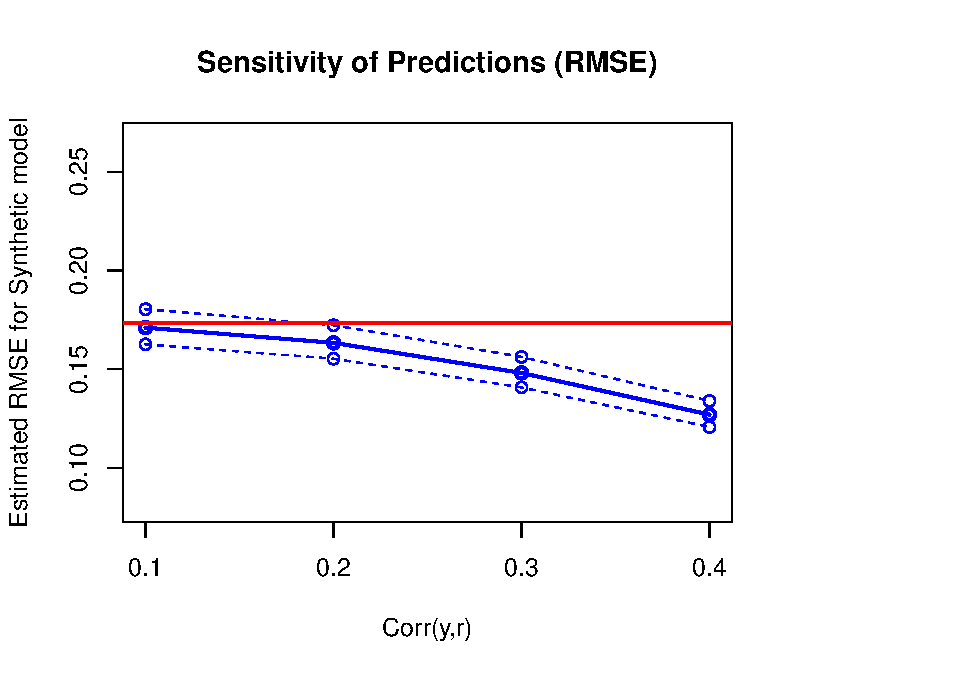
\includegraphics{sensitivity_analysis_files/figure-latex/unnamed-chunk-8-1.pdf}

\hypertarget{r-squared}{%
\subsubsection{R squared}\label{r-squared}}

In the following chunk of code we construct confidence intervals for the
\(R^2\). The standard error of the \(R^2\) can be derived as follows:
\begin{equation}
se_{R^2}=\sqrt{\frac{4R^2(1-R^2)^2(n-k-1)^2}{(n^2-1)(n+3)}} 
\end{equation} where \(k\) is the number of predictors. See Cohen et al.
(2003), Applied Multiple Regression/Correlation Analysis for the
Behavioral Sciences, p.~88 for details.

\begin{Shaded}
\begin{Highlighting}[]
\NormalTok{n =}\StringTok{ }\KeywordTok{nrow}\NormalTok{(train_bart}\OperatorTok{$}\NormalTok{X)}
\NormalTok{k =}\StringTok{ }\KeywordTok{ncol}\NormalTok{(train_bart}\OperatorTok{$}\NormalTok{X)}
\NormalTok{r2 =}\StringTok{ }\NormalTok{sensitivity}\OperatorTok{$}\StringTok{`}\DataTypeTok{Rsquared original model}\StringTok{`}
\NormalTok{ub_new <-}\StringTok{ }\NormalTok{lb_new <-}\StringTok{ }\KeywordTok{c}\NormalTok{()}
\ControlFlowTok{for}\NormalTok{(j }\ControlFlowTok{in}\NormalTok{ (}\DecValTok{1}\OperatorTok{:}\KeywordTok{length}\NormalTok{(sensitivity}\OperatorTok{$}\StringTok{`}\DataTypeTok{Rsquared synthetic model}\StringTok{`}\NormalTok{)))\{}
\NormalTok{  r2_new =}\StringTok{ }\NormalTok{sensitivity}\OperatorTok{$}\StringTok{`}\DataTypeTok{Rsquared synthetic model}\StringTok{`}\NormalTok{[j]}
\NormalTok{  se_r2_new <-}\StringTok{ }\KeywordTok{sqrt}\NormalTok{((}\DecValTok{4}\OperatorTok{*}\NormalTok{r2_new}\OperatorTok{*}\NormalTok{(}\DecValTok{1}\OperatorTok{-}\NormalTok{r2_new)}\OperatorTok{^}\DecValTok{2}\OperatorTok{*}\NormalTok{(n}\OperatorTok{-}\NormalTok{k}\DecValTok{-1}\NormalTok{)}\OperatorTok{^}\DecValTok{2}\NormalTok{)}\OperatorTok{/}\NormalTok{((n}\OperatorTok{^}\DecValTok{2-1}\NormalTok{)}\OperatorTok{*}\NormalTok{(n}\OperatorTok{+}\DecValTok{3}\NormalTok{)))}
\NormalTok{  ub_new[j] =}\StringTok{ }\NormalTok{r2_new }\OperatorTok{+}\StringTok{ }\FloatTok{2.58}\OperatorTok{*}\NormalTok{se_r2_new }\CommentTok{# Change Z-score for difference alpha levels}
\NormalTok{  lb_new[j] =}\StringTok{ }\NormalTok{r2_new }\OperatorTok{-}\StringTok{ }\FloatTok{2.58}\OperatorTok{*}\NormalTok{se_r2_new }\CommentTok{# Change Z-score for difference alpha levels}
\NormalTok{\}}

\KeywordTok{par}\NormalTok{(}\DataTypeTok{mar=}\KeywordTok{c}\NormalTok{(}\FloatTok{5.1}\NormalTok{, }\FloatTok{4.1}\NormalTok{, }\FloatTok{4.1}\NormalTok{, }\FloatTok{8.1}\NormalTok{), }\DataTypeTok{xpd=}\OtherTok{TRUE}\NormalTok{)}
\KeywordTok{plot}\NormalTok{(sensitivity}\OperatorTok{$}\StringTok{`}\DataTypeTok{Rsquared synthetic model}\StringTok{`}\NormalTok{,}
     \DataTypeTok{main =} \StringTok{"Sensitivity of Predictions (R Squared)"}\NormalTok{,}
     \DataTypeTok{xlab =} \StringTok{"Corr(y,r)"}\NormalTok{,}
     \DataTypeTok{ylab =} \StringTok{"Estimated R Squared"}\NormalTok{, }
     \DataTypeTok{xaxt=}\StringTok{'n'}\NormalTok{,}
     \DataTypeTok{type =} \StringTok{"o"}\NormalTok{,}
     \DataTypeTok{col =} \StringTok{"blue"}\NormalTok{,}
     \DataTypeTok{lwd =} \DecValTok{2}\NormalTok{,}
     \DataTypeTok{ylim=}\KeywordTok{c}\NormalTok{(r2}\FloatTok{-0.5}\NormalTok{,r2}\FloatTok{+0.5}\NormalTok{))}
\KeywordTok{par}\NormalTok{(}\DataTypeTok{xpd =} \OtherTok{FALSE}\NormalTok{)}
\KeywordTok{lines}\NormalTok{(lb_new, }\DataTypeTok{col =} \StringTok{"blue"}\NormalTok{, }\DataTypeTok{lty=}\DecValTok{2}\NormalTok{, }\DataTypeTok{type =} \StringTok{"o"}\NormalTok{)}
\KeywordTok{lines}\NormalTok{(ub_new, }\DataTypeTok{col =} \StringTok{"blue"}\NormalTok{, }\DataTypeTok{lty=}\DecValTok{2}\NormalTok{, }\DataTypeTok{type =} \StringTok{"o"}\NormalTok{)}
\KeywordTok{abline}\NormalTok{(}\DataTypeTok{h=}\NormalTok{ r2, }\DataTypeTok{col =} \StringTok{"red"}\NormalTok{, }\DataTypeTok{lwd =} \DecValTok{2}\NormalTok{)}
\KeywordTok{axis}\NormalTok{(}\DecValTok{1}\NormalTok{, }\DataTypeTok{at=}\DecValTok{1}\OperatorTok{:}\NormalTok{(}\KeywordTok{length}\NormalTok{(sensitivity}\OperatorTok{$}\StringTok{`}\DataTypeTok{Rsquared synthetic model}\StringTok{`}\NormalTok{)), }
     \DataTypeTok{labels=}\KeywordTok{c}\NormalTok{(}\KeywordTok{seq}\NormalTok{(}\FloatTok{0.1}\NormalTok{,}\FloatTok{0.4}\NormalTok{,}\FloatTok{0.1}\NormalTok{)))}
\end{Highlighting}
\end{Shaded}

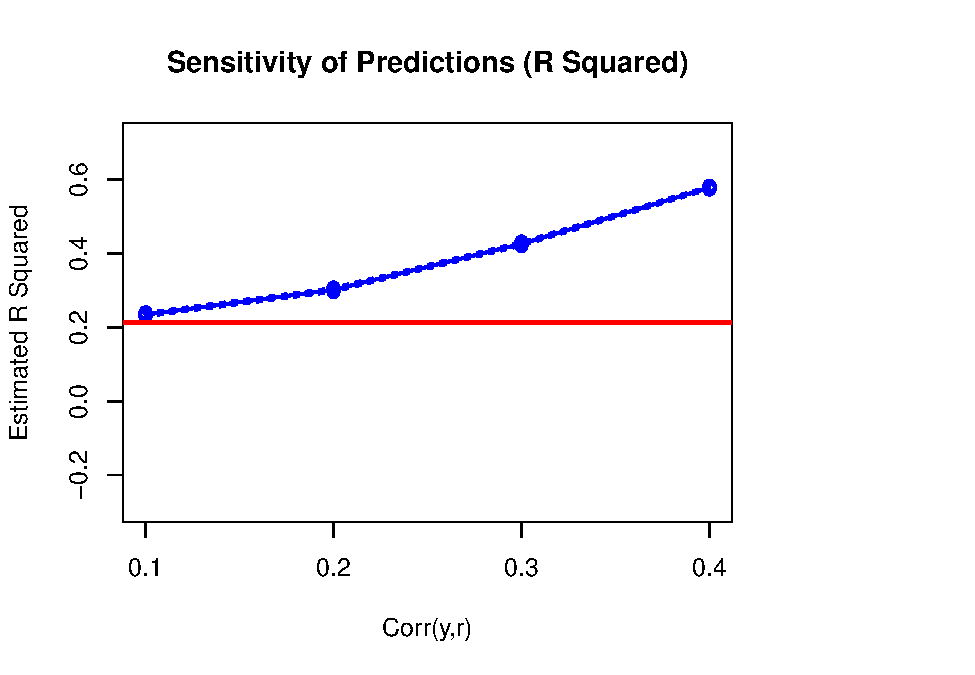
\includegraphics{sensitivity_analysis_files/figure-latex/unnamed-chunk-9-1.pdf}

\hypertarget{standardized-difference-in-means}{%
\section{Standardized Difference in
Means}\label{standardized-difference-in-means}}

Moreover, the standardized difference in the means between
\(\hat{p}(Y_i =1 |X_i = x)\) and \(\hat{p}(Y_i = 1|X_i = x, R_i = r)\)
is not significant in all the cases.

Standardized differences in mean and their standard deviations from
Cohen (1988, p.44).

\begin{Shaded}
\begin{Highlighting}[]
\CommentTok{# Standardized difference in means}
\NormalTok{diff.means <-}\StringTok{ }\NormalTok{ppd_mean }\OperatorTok{-}\StringTok{ }\NormalTok{new_ppd_mean}
\NormalTok{standard.diff.means <-}\StringTok{  }\NormalTok{(diff.means)}\OperatorTok{/}\KeywordTok{sqrt}\NormalTok{((ppd_sd}\OperatorTok{^}\DecValTok{2} \OperatorTok{+}\StringTok{ }\NormalTok{new_ppd_sd}\OperatorTok{^}\DecValTok{2}\NormalTok{)}\OperatorTok{/}\DecValTok{2}\NormalTok{)}

\CommentTok{# 99% CI (t-student distribution)}
\NormalTok{x0 <-}\StringTok{ }\NormalTok{standard.diff.means }\OperatorTok{-}\StringTok{ }\FloatTok{2.58} \OperatorTok{*}\StringTok{ }
\StringTok{  }\KeywordTok{sqrt}\NormalTok{((ppd_sd}\OperatorTok{^}\DecValTok{2} \OperatorTok{+}\StringTok{ }\NormalTok{new_ppd_sd}\OperatorTok{^}\DecValTok{2}\NormalTok{)}\OperatorTok{/}\DecValTok{2}\NormalTok{)}
\NormalTok{x1 <-standard.diff.means  }\OperatorTok{+}\StringTok{ }\FloatTok{2.58} \OperatorTok{*}\StringTok{ }
\StringTok{  }\KeywordTok{sqrt}\NormalTok{((ppd_sd}\OperatorTok{^}\DecValTok{2} \OperatorTok{+}\StringTok{ }\NormalTok{new_ppd_sd}\OperatorTok{^}\DecValTok{2}\NormalTok{)}\OperatorTok{/}\DecValTok{2}\NormalTok{)}
\end{Highlighting}
\end{Shaded}

This can be seen from the plot of the Standardized difference in means
for the probabilities predicted by the two models.

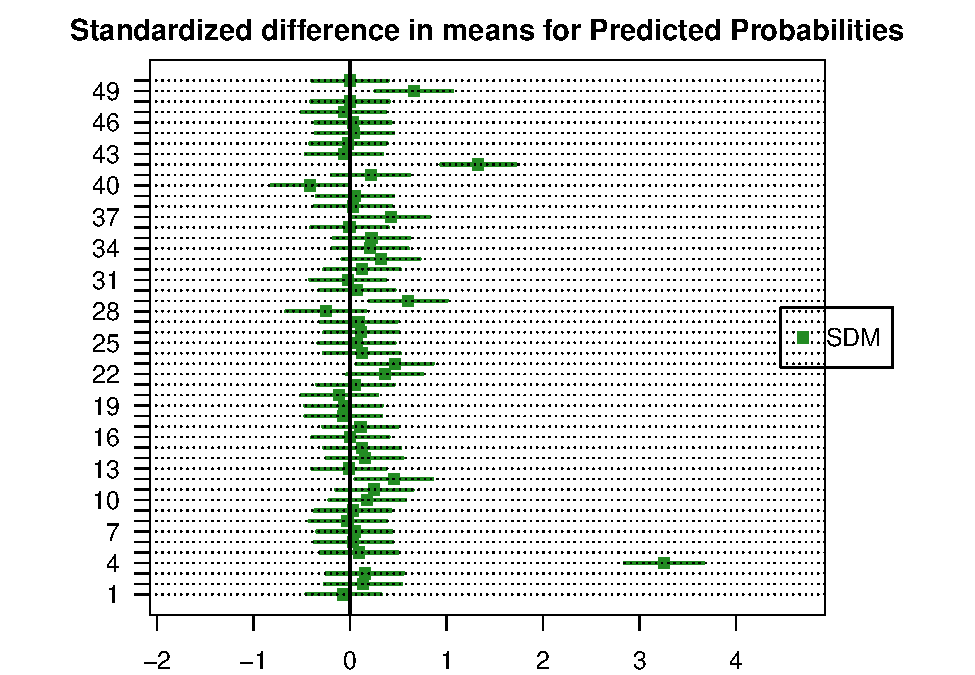
\includegraphics{sensitivity_analysis_files/figure-latex/unnamed-chunk-12-1.pdf}


\end{document}
